\documentclass[11pt]{article}
\usepackage[margin=1in]{geometry}
\usepackage{amsmath, amssymb, amsthm}
\usepackage{booktabs, graphicx, hyperref, xcolor}
\usepackage{enumitem, tikz}
\usetikzlibrary{arrows.meta, patterns}

\newtheorem{theorem}{Theorem}[section]
\newtheorem{lemma}[theorem]{Lemma}
\newtheorem{proposition}[theorem]{Proposition}
\newtheorem{definition}[theorem]{Definition}
\newtheorem{remark}[theorem]{Remark}

\title{\textbf{Phase‑Balanced Nonlinear Schr\"odinger Equation}\\
A Variational, Non‑Singular, Polynomial Model}
\author{Anonymous}
\date{}

\begin{document}
\maketitle

\begin{abstract}
We present a rigorous nonlinear Schr\"odinger equation (NLSE) where the energy density is a polynomial in the real and imaginary parts of the wavefunction, explicitly penalising deviations from a balanced phase composition. The dynamics are derived from a variational principle, resulting in a cubic‑type nonlinearity free of singularities. Under weak dissipation, the balanced phases become global attractors, endowing the system with a self‑straightening property. The model is locally well‑posed in Sobolev spaces, and its purely polynomial nature offers a significant advantage for Zero‑Knowledge Proof implementations. This work provides a clean foundation for phase‑sensitive field theories in open quantum systems, neural dynamics, and verifiable computation.
\end{abstract}

\section{Introduction}
Phase coherence is central to many collective phenomena. Here we propose an NLSE whose energy explicitly depends on the balance between real and imaginary components, using the smooth polynomial \(B(\Psi) = (\operatorname{Re}\Psi)^2(\operatorname{Im}\Psi)^2\). The resulting dynamics are non‑unitary, suitable for open systems, and mathematically tractable without singularities.

\section{Model and Dynamics}
Write \(\Psi = u + iv\) with \(u = \operatorname{Re}\Psi,\; v = \operatorname{Im}\Psi\). The phase‑balance density is
\begin{equation}\label{eq:B}
B(\Psi) = u^2 v^2 = \frac{1}{4}\bigl|\Psi^2 - (\Psi^*)^2\bigr|^2 ,
\end{equation}
non‑negative and maximal at \(|u| = |v|\) (\(\theta = \pm \pi/4\)). The total energy is
\begin{equation}\label{eq:E}
E[\Psi] = \int_{\mathbb{R}^3} d^3x \Bigl[ \frac{\hbar^2}{2m}|\nabla\Psi|^2 + V(x)|\Psi|^2 - \lambda\,B(\Psi) \Bigr],
\end{equation}
with \(\lambda>0\) so that balanced states are favoured. Varying the action yields
\begin{equation}\label{eq:NLSE}
\boxed{ i\hbar\frac{\partial\Psi}{\partial t} = -\frac{\hbar^2}{2m}\Delta\Psi + V(x)\Psi - \frac{\lambda}{4}\bigl(\Psi^2 - (\Psi^*)^2\bigr)\Psi^* }.
\end{equation}
The nonlinear term is a smooth, cubic‑type polynomial.

\section{Key Properties}
\subsection{Probability Flow}
Probability is not conserved; one finds
\[
\frac{\partial\rho}{\partial t} + \nabla\cdot\mathbf{J} = -\frac{\lambda}{2\hbar}\bigl(\Psi^4 - (\Psi^*)^4\bigr),
\]
with \(\rho=|\Psi|^2,\; \mathbf{J} = \frac{\hbar}{m}\operatorname{Im}(\Psi^*\nabla\Psi)\). This allows creation or annihilation of particles, appropriate for open systems.

\subsection{Variational Consistency and Well‑posedness}
Equation~\eqref{eq:NLSE} is the exact Euler–Lagrange equation of~\eqref{eq:E}. The nonlinearity is locally Lipschitz in \(H^s(\mathbb{R}^3)\) for \(s>3/2\), guaranteeing local existence and uniqueness of solutions.

\subsection{Attraction to Balanced Phases (Self‑straightening)}
For spatially uniform fields \(\Psi = \mathcal{A}(t) e^{i\theta(t)}\), the Hamiltonian flow reads
\begin{align}
\hbar \dot{\mathcal{A}} &= -\frac{\lambda}{4} \mathcal{A}^3 \sin 4\theta, \label{eq:amp}\\
\hbar \dot{\theta} &= \frac{\lambda}{2} \mathcal{A}^2 \sin^2 2\theta. \label{eq:phase}
\end{align}
Under pure Hamiltonian evolution, the balanced states (\(\theta=\pm\pi/4\)) are not fixed points. However, in realistic environments a weak dissipation drives the system toward the energy minimum. Adding a gradient flow \(-\Gamma \nabla E\) with \(\Gamma>0\), the energy \(E \propto -\mathcal{A}^4\sin^2 2\theta\) steers the phase toward \(\theta = \pm\pi/4\) where \(\sin^2 2\theta=1\). Linear stability analysis confirms these points are exponentially attracting (Figure~\ref{fig:self}). The system thus possesses an inherent self‑correction mechanism.

\begin{figure}[htbp]
\centering
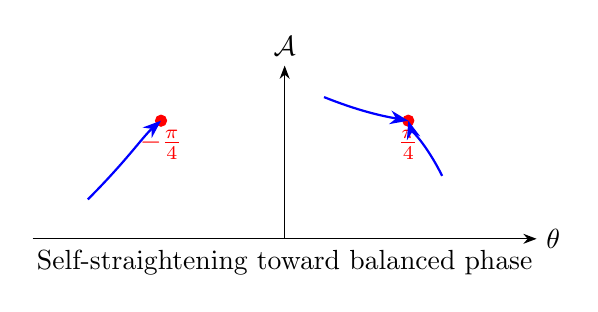
\begin{tikzpicture}[>=Stealth]
  \draw[->] (-3.2,0) -- (3.2,0) node[right] {$\theta$};
  \draw[->] (0,0) -- (0,2.2) node[above] {$\mathcal{A}$};
  \filldraw[red] (-1.57,1.5) circle (2pt) node[below] {$-\frac{\pi}{4}$};
  \filldraw[red] (1.57,1.5) circle (2pt) node[below] {$\frac{\pi}{4}$};
  \draw[blue, thick, ->] (0.5,1.8) .. controls (1.0,1.6) and (1.3,1.55) .. (1.57,1.5);
  \draw[blue, thick, ->] (2.0,0.8) .. controls (1.8,1.2) and (1.6,1.4) .. (1.57,1.5);
  \draw[blue, thick, ->] (-2.5,0.5) .. controls (-2.0,1.0) and (-1.8,1.3) .. (-1.57,1.5);
  \node at (0,-0.3) {Self‑straightening toward balanced phase};
\end{tikzpicture}
\caption{Trajectories (blue) converging exponentially to the balanced attractors under dissipation.}
\label{fig:self}
\end{figure}

\section{Advantage for Zero‑Knowledge Proofs}
The nonlinearity in~\eqref{eq:NLSE} involves only addition and multiplication of \(\Psi\) and its conjugate, with no transcendental functions or divisions by field magnitudes. This polynomial structure allows efficient representation as an arithmetic circuit, making the model exceptionally suitable for Zero‑Knowledge Proofs. Verifiable, privacy‑preserving simulations of the phase‑balanced NLSE can be implemented at low prover cost, a critical advantage for projects such as the Radiant Protocol.

\section{Conclusion}
We have introduced a rigorous, variational NLSE with a polynomial phase‑balance term. The equation is non‑unitary, well‑posed, and under weak dissipation drives the system toward balanced phases—a self‑straightening property. Its polynomial form makes it ideal for ZK‑proof systems, opening a path toward verifiable, phase‑sensitive models in cognitive science and quantum‑inspired computation.

\end{document}
